\chapter{Introduction}
\label{chapter:Introduction}

The Internet today is a vast source of information curated by real people. In recent times, the popularity of websites like Twitter, Reddit, and Wordpress has shown that every day, more and more people are getting comfortable with expressing their inner feelings on the web, irrespective of whether they feel good or bad. Negative feelings expressed this way provide an important indicator of what might be going wrong in their lives, or what may ultimately lead up to something more tragic or even terminal. In some cases, factors leading to suicide can be identified early on by looking at the physical and verbal behavior of the person under consideration. Public availability of a larger set of data that may contain content posted by emotionally distressed people, and non-availability of a system that can analyze such data to find such people is a clear disconnect. This thesis attempts to bridge this gap by applying machine learning techniques to build a system that is able to find instances of emotionally distressed content on the Internet. This can then serve as a first step towards providing further help to such people, possibly in the form of human intervention.

\section{Public emotion on the Internet}
There have been some studies conducted on the measure of happiness on Twitter as a function of time. One such work \cite{dodds2011temporal} performed the analysis on a dataset comprising of 46 billion words collected from Twitter over a period of 33 months, and showed that over time, the amount of negative emotions being expressed on Twitter has been on the rise. Visualization of a part of their results can be seen in Figure~\ref{fig:twitter_happiness}. The words that were assigned negative emotions in this study included \emph{``death''}, \emph{``hate''}, and even \emph{``suicide''}. A study conducted at Cornell University \cite{golder2011diurnal} analyzes the effects of the time of the day on the moods of people, all from a dataset collected from Twitter. Studies like these show that in recent times, people are getting more and more comfortable with expressing their emotions on Twitter.\\

\begin{figure}
    \centering
    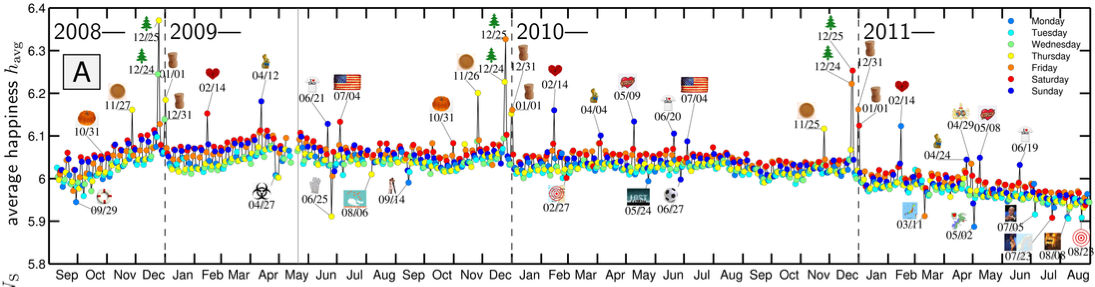
\includegraphics[width=\textwidth]{twitter_happiness.png}
    \caption{A plot of happiness on Twitter as a function of time}
    \label{fig:twitter_happiness}
\end{figure}

In the past, there have been very public instances of people posting updates about how they are feeling right before they have committed suicide. Figure~\ref{fig:twitter_kcs} shows the last tweet of Twitter user \href{http://twitter.com/CapitalSTEEZ\_}{KING CAPITAL \$TEEZ} before committing suicide. Similarly, Figure~\ref{fig:twitter_fe} shows the series of updates posted by Twitter user \href{http://twitter.com/Freddy\_E}{Freddy\_E} prior to committing suicide.\\

\begin{figure}
    \centering
    
\includegraphics[width=0.8\textwidth]{twitter_kcs.png}
    \caption{The last tweet of Twitter user \href{http://twitter.com/CapitalSTEEZ\_}{KING CAPITAL \$TEEZ}}
    \label{fig:twitter_kcs}
\end{figure}

\begin{figure}
    \centering
    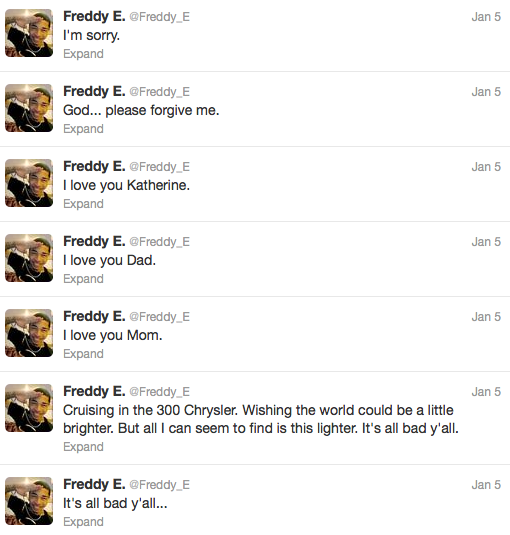
\includegraphics[width=0.8\textwidth]{twitter_fe.png}
    \caption{Last few updates posted by Twitter user \href{http://twitter.com/Freddy\_E}{Freddy\_E}}
    \label{fig:twitter_fe}
\end{figure}

While these were the instances where the person under concern had a number of followers on their Twitter accounts, it is not unreasonable to assume that there are countless other instances where similar content was posted but did not reach a lot of people because the account did not have many followers. Lives in such cases are lost, partially because there was no one to help them. A system that can proactively look for such content online will go a long way in solving this problem.

\section{Problem Definition}
A large portion of the nearly one million people who die every year from suicide includes young people. In recent times, these people have started to express their inner feelings on the web, on websites like Twitter, Wordpress, Reddit (Figure~\ref{fig:reddit_happy} and Figure~\ref{fig:reddit_suicidewatch}), and many others. Suicide is a medical condition that has the potential to be detected early on, by observing the physical and verbal behavior of the person under concern. The work presented in this thesis exploits these two facts, and attempts to build a system that can monitor the public feed of Internet websites such as Twitter (on which people post about what they feel) and detect the content that may have been posted by a person under emotional distress.\\

\begin{figure}[t!]
    \centering
    
\includegraphics[width=0.8\textwidth]{reddit_happy.png}
    \caption{\href{http://www.reddit.com/r/happy}{``/r/happy''}, the section of the website Reddit \cite{reddit} where people post content when they are happy and want to share it with everyone else.}
    \label{fig:reddit_happy}
\end{figure}

\begin{figure}[t!]
    \centering
    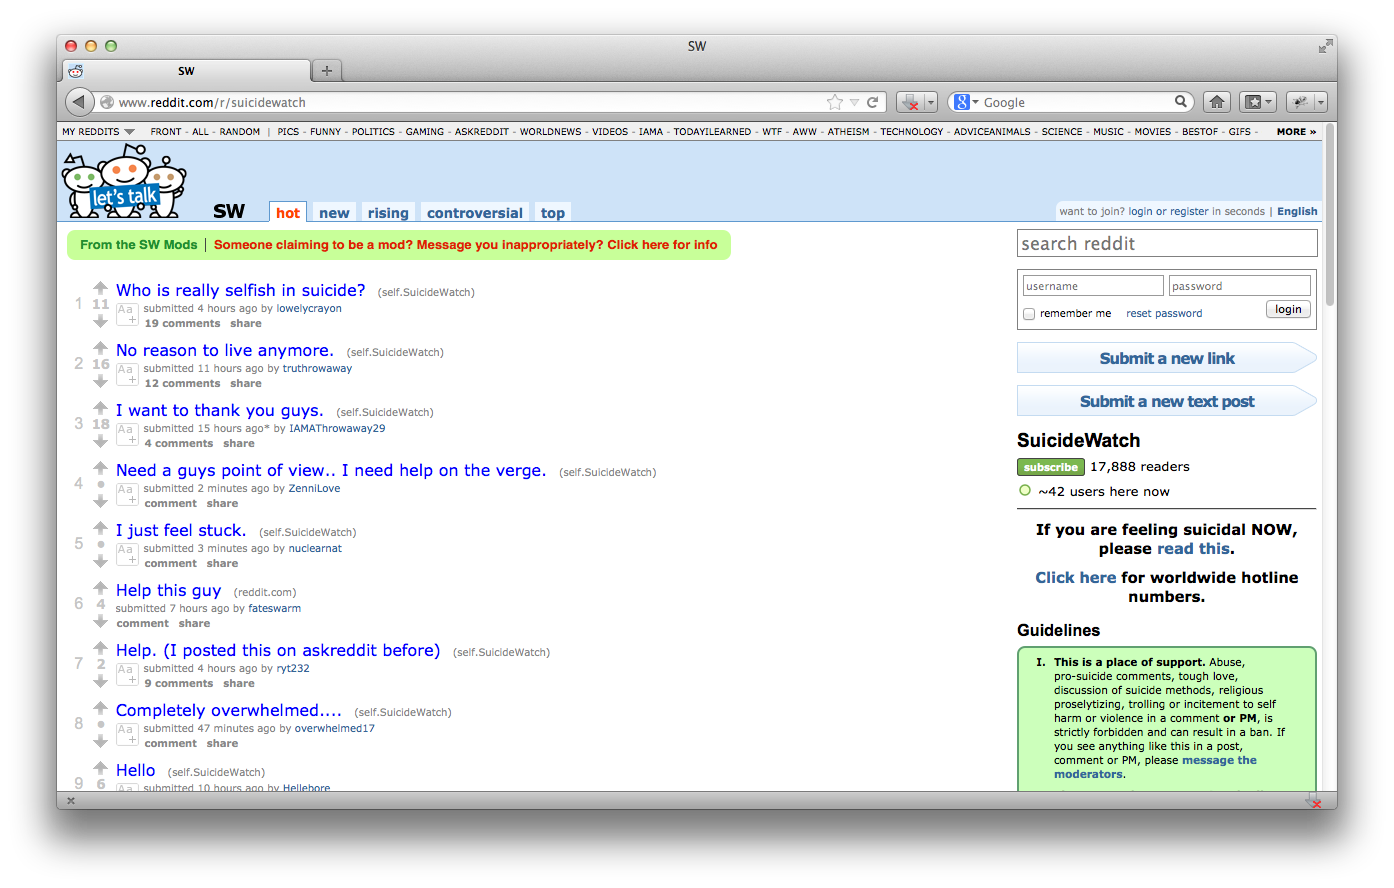
\includegraphics[width=0.8\textwidth]{reddit_suicidewatch.png}
    \caption{\href{http://www.reddit.com/r/suicidewatch}{``/r/suicidewatch''}, the section of Reddit \cite{reddit} where people post when they are depressed, or are on the verge of taking their own lives.}
    \label{fig:reddit_suicidewatch}
\end{figure}

Pointing out the exact phrases which lead one to believe that a person may be under some degree of emotional distress is a problem best handled by psychologists and linguists. Even though prediction with machine learning algorithms is less sophisticated than human classification, it is known (and also presented in this thesis) that such techniques can identify and categorize the sentiment of a piece of text to a reasonable accuracy. A person may be under emotional distress if he/she posts content which is indicative of sentiments and/or actions like depression, suicide, loneliness, and helplessness. During the work performed in this thesis, the following two categories of phrases were found indicative of whether or not a person needs help.

\begin{itemize}
    \item{\textbf{Direct} Phrases such as \emph{``thoughts of suicide make me happy''}, \emph{``I have a rope around my neck''} or \emph{``my suicide note''} indicate in a very straightforward manner that the author is not only depressed, but is also on the path of taking his/her own life. Such phrases are very direct indicators of the emotional condition of the person.}
    \item{\textbf{Indirect} Phrases such as \emph{``I don't know anything anymore''} or \emph{``Need someone to talk to''} or \emph{``Please help''} indicate that the person who is posting such content does not necessarily want to kill themselves yet, but they are not in a very good emotional condition either. Such words indicate that this person is under depression, or is feeling lonely. Even though they may not be suicidal yet, such a dramatic and tragic event might be the next step in their lives.}
\end{itemize}

Both the category of phrases indicate that the emotional health of the person under consideration is not normal, and may need attention.\\

The work presented in this thesis tackles this problem by following a two-step approach. In the first step, various text classification algorithms are explored and evaluated that could be a good fit for the problem at hand (identification of text which may or may not have been posted by a depressed person). In the second step, these algorithms are used to build a system that proactively looks for content on the Internet (on places like Twitter), and identifies people who have been posting emotionally distressed content. The system also allows for making improvements to its abilities by tapping into crowd intelligence, which distinguishes the problem being addressed from normal text classification problems. A detailed explanation of this particular aspect can be found in Chapter~\ref{chapter:Experiments}. This system then serves as a first step towards extending a helpful hand to people who need it.
